
%(BEGIN_QUESTION)
% Copyright 2008, Tony R. Kuphaldt, released under the Creative Commons Attribution License (v 1.0)
% This means you may do almost anything with this work of mine, so long as you give me proper credit

Identify the states of both light bulbs when the normally-open pressure switch contact {\it opens}:

$$\includegraphics[width=15.5cm]{i03205x01.eps}$$

Assuming that the green light bulb signifies a ``good'' process condition and the red light bulb signifies a ``bad'' (alarm) process condition, determine whether this is a {\it low-pressure} alarm or a {\it high pressure} alarm circuit.

\vfil 

Hint: remember that the ``normal'' status of a switch is defined as the status of {\it minimum stimulus}: when the switch is exposed to the lowest possible degree of process stimulation (in this particular case, to the lowest possible pressure).

\underbar{file i03205}
\eject
%(END_QUESTION)





%(BEGIN_ANSWER)

This is a graded question -- no answers or hints given!
 
%(END_ANSWER)





%(BEGIN_NOTES)

Remember that the ``normal'' status for any switch contact is its ``resting'' state, where there is no stimulus applied to it.  Since this is a pressure switch, the stimulus in question is fluid pressure.  Thus, this switch will be in its normal state when there is low (or no) fluid pressure.

Following this logically, we will analyze what happens in this condition with no or low presusre.  When the normally-open pressure switch contact opens due to there being low or no pressure applied to the switch, the relay de-energizes, closing the normally-closed relay contact to turn the green light on and opening the normally-open relay contact to turn the red light off.  Thus, the green light energizes and the red light de-energizes whenever the gas pressure is low.

\vskip 10pt

Therefore, this circuit functions as a {\it high-pressure} alarm, turning the red light bulb on and the green light bulb off if the process pressure ever rises above the switch's trip value (forcing the pressure switch out of its normal state and into its {\it actuated} state).

%INDEX% Pictorial circuit review (relay circuit)

%(END_NOTES)


